% !TeX root = ../defense.tex

\section{Results, Conclusion and Further Work}
\frame{\sectionpage}

\begin{frame}{Data Distribution}
    The data obtained by executing all the orderings for the query plan on Linear road data, resulted in the following frequencies for optimal orderings.
    \begin{figure}
        \centering
        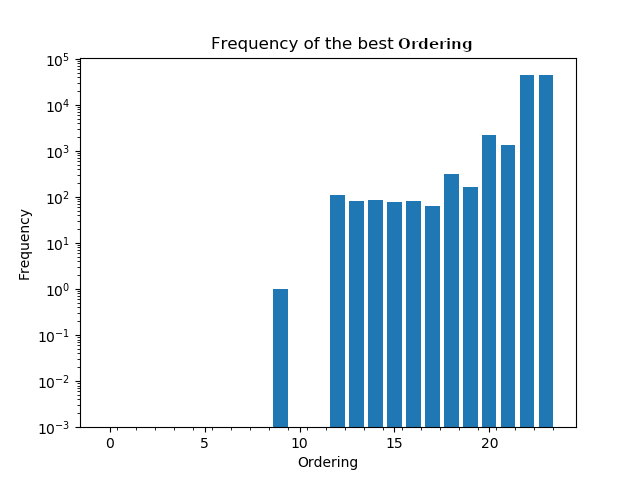
\includegraphics[scale=0.375]{totalb1.png}\\
        \caption{This figure shows the frequency distribution of the number of cases where each move is optimal}
        \label{fig:totalb1}
    \end{figure}
\end{frame}


\begin{frame}{Data Distribution}
    While training and testing the DQN model, we divided the total data into a $70:30$ for training and testing purposes respectively.
    \begin{figure}
        \centering
        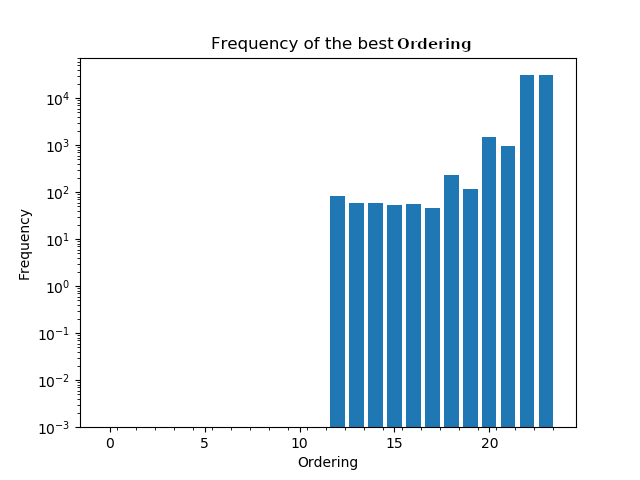
\includegraphics[scale=0.375]{trainingb1.png}\\
        \caption{This figure shows the frequency distribution of cases where each move is optimal in the training dataset}
        \label{fig:trainingb1}
    \end{figure}
\end{frame}

\begin{frame}{Data Distribution}
    While training and testing the DQN model, we divided the total data into a $70:30$ for training and testing purposes respectively.
    \begin{figure}
        \centering
        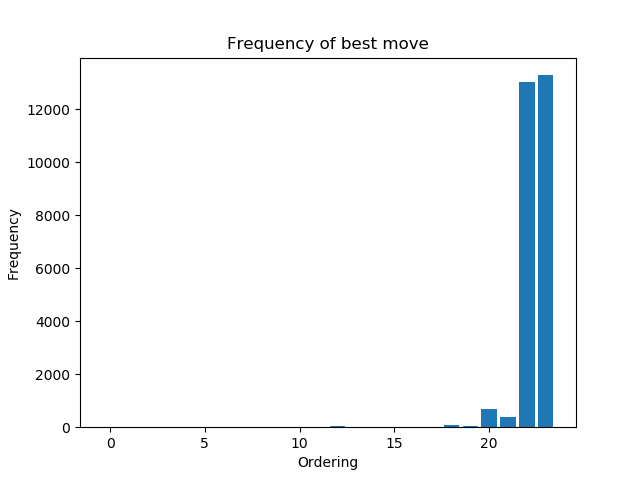
\includegraphics[scale=0.375]{testingb1.png}\\
        \caption{This figure shows the frequency distribution of cases where each move is optimal in the testing dataset}
        \label{fig:testingb1}
    \end{figure}
\end{frame}


\begin{frame}{Confusion Matrix}
    The predictions on trained model lead to the following confusion matrix.
    \begin{figure}
        \centering
        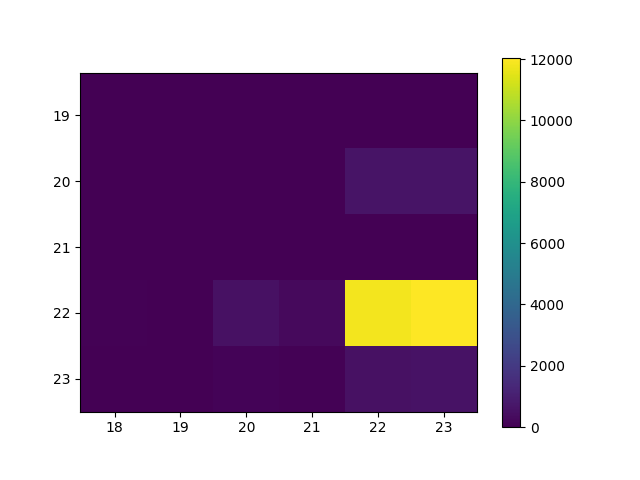
\includegraphics[scale=0.3]{cm3.png}\\
        \caption{DQN predictions visualized as confusion matrix}
        \label{fig:dqn_r2_1}
    \end{figure}
\end{frame}

\begin{frame}{Predictions}
    Some of the cases we were able to predict the correct answers.
    \begin{figure}
        \centering
        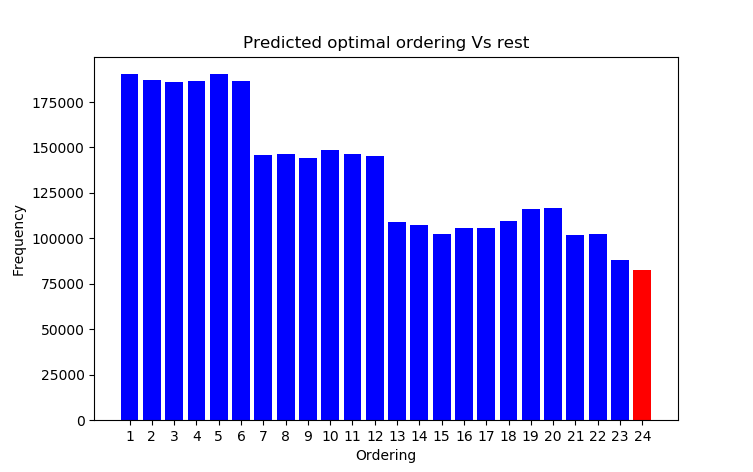
\includegraphics[scale=0.4]{operations1.png}\\
        \caption{The figure shows the log$_{10}$(number of operations) required to execute the query depending on the ordering of the selection operators chosen. The predicted optimal ordering is shown in red.}
        \label{fig:operations1}
    \end{figure}
\end{frame}

\begin{frame}{Predictions}
    Some of the cases we were able to predict the correct answers.
    \begin{figure}
        \centering
        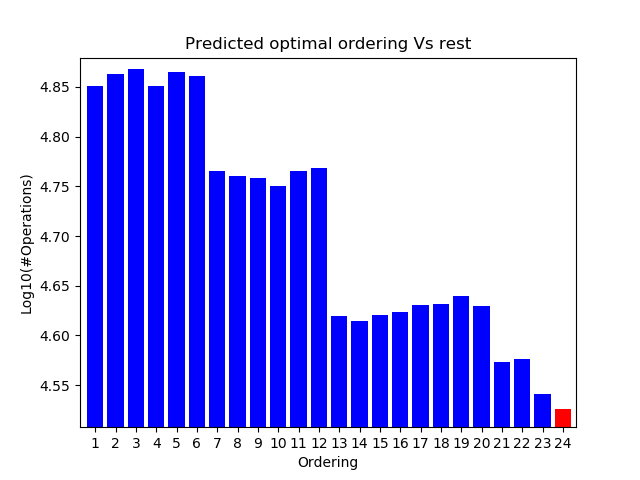
\includegraphics[scale=0.4]{operations2.png}\\
        \caption{The figure shows the log$_{10}$(number of operations) required to execute the query depending on the ordering of the selection operators chosen. The predicted optimal ordering is shown in red.}
        \label{fig:operations2}
    \end{figure}
\end{frame}



